The algorithm and the visualization of the semantically structured docids are depicted respectively in \ref{alg:semanticids} and \ref{fig:ssdocids-visualization}.


\begin{algorithm}[H]
    \label{alg:semanticids}
    \caption{Generating Semantically Structured Identifiers}
    \begin{algorithmic}[1]
    \Require Document embeddings $X_{1:N}$, where $X_i \in \mathbb{R}^d$ generated by a small 8-layer BERT model with $c=100$
    \Ensure Corresponding docid strings $J_{1:N}$
    \Function{GENERATE\_SEMANTIC\_IDS}{$X_{1:N}$}
        \State $C_{1:10} \gets \Call{Cluster}{X_{1:N},\, k=10}$ \# k-means clustering
        \State $J \gets$ empty list
        \For{$i \gets 0$ to $9$}
            \State $J_{\text{current}} \gets [i] \times |C_{i+1}|$
            \If{$|C_{i+1}| > c$} \# recursion if there are more than c documents
                \State $J_{\text{rest}} \gets \Call{GENERATE\_SEMANTIC\_IDS}{C_{i+1}}$
            \Else
                \State $J_{\text{rest}} \gets [0,\dots,|C_{i+1}| - 1]$ \# assign arbitrary number from 0 to $c-1$
            \EndIf
            \State $J_{\text{cluster}} \gets \Call{elementwise\_Str\_Concat}{J_{\text{current}},\,J_{\text{rest}}}$
            \State $J \gets J.\Call{append\_elements}{J_{\text{cluster}}}$ \# Append all elements of $J_{\text{cluster}}$ to $J$
        \EndFor
        \State $J \gets \Call{reorder\_to\_Original}{J,\,X_{1:N},\,C_{1:10}}$
        \State \Return $J$
    \EndFunction
    \end{algorithmic}
\end{algorithm}


\begin{figure*}
    \centering
    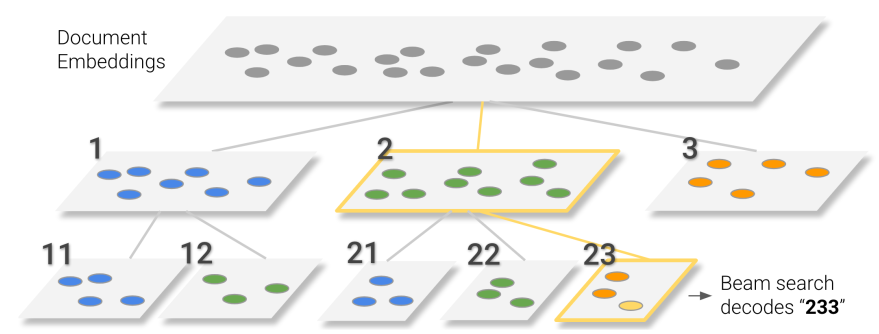
\includegraphics[width=0.75\textwidth]{../figs/ssdocid.png}
    \caption{Visualization of the Semantically Structured Docids tree for extracting identifiers from latent space.}
    \label{fig:ssdocids-visualization}
  \end{figure*}

